\section{Evaluation}
\label{s:eval}

To verify the effectiveness of our approach, we evaluate \sys in
various aspects.
%
Specifically, we 1) demonstrate the practicality of \sys by providing
newly found concurrency bugs in the Linux
kernel~(\autoref{ss:realworldbugs}),
%
2) provide comprehensive performance characteristics of \sys (\eg,
throughput and overheads)~(\autoref{ss:characteristics}) and,
%
3) compare \sys against prior concurrency fuzzing
techniques~(\autoref{ss:comparison}).

\subsection{Finding Real-world Concurrency Bugs}
\label{ss:realworldbugs}

In order to demonstrate the practicality of \sys, we run \sys to
discover concurrency bugs in the latest Linux kernel.

\begin{table*}[t]
  \resizebox{\linewidth}{!}{
  \begin{tabular}{r l l l l}
  \toprule
    Crash ID & Kernel Version (Commit) & Subsystem & Crash Type & Crash Summary \\
  \midrule
  1 \\
  \midrule
  2 \\ 
  \midrule
  3 \\
  \midrule
  4 \\
  \midrule
  5 \\
  \midrule
  6 \\
  \midrule
  7 \\
  \midrule
  8 \\
  \midrule
  9 \\
  \midrule
  10 \\
  \midrule
  11 \\
  \midrule
  12 \\
  \midrule
  13 \\
  \midrule
  14 \\
  \midrule
  15 \\
  \midrule
  16 \\
  \midrule
  17 \\
  \midrule
  18 \\
  \midrule
  19 \\
  \midrule
  20 \\
  \midrule
  21 \\
  \bottomrule
  \end{tabular}
}

%%% Local Variables:
%%% mode: latex
%%% TeX-master: "../p.tex"
%%% End:

  \centering
  \caption{List of concurrency bugs newly discovered by \sys. The
    \texttt{Recurrent} column denotes that a crash was previously
    addressed but reoccurs even after its patch is applied.}
  \label{table:newbugs}
\end{table*}

\PP{Experimental setup.}
%
To discover new concurrency bugs, we evaluate \sys on a two-socket
machine equipped with Intel(R) Xeon(R) CPU E5-2683 v4 @ 2.10GHz (40M
cache) and 512\GB of RAM.
%
This machine provides 32 total cores and 64 total threads, and runs
Ubuntu Server 20.04.4 LTS on Linux 5.4.143 as a host operating system.
%
During our experiments, we launch 32 virtual machines (VMs) where each
VM is equipped with four vCPUs and 8\GB memory.

To build a guest kernel, we use a kernel configuration used by
\texttt{Syzkaller}~\cite{syzkaller} so that \texttt{Syzkaller} and
\sys search for bugs in similar kernel modules/subsystems.
%
We run intermittently \sys for approximately two monts on latest
versions of the Linux kernel ranging from 5.19-rc2 to 6.0-rc7.


\PP{Newly found concurrency bugs.}
%
During our evaluation, \sys discovers 83 unique crash titles including
ones that \texttt{Syzkaller} also finds. Among them, \totalbugs are
newly identified as harmful concurrency bugs as summarized in
\autoref{table:newbugs}.
%
This table shows that \sys is able to find bugs across the entire
kernel from specific device drivers~(\eg, \texttt{\#1}, and
\texttt{\#6}) to various network subsystems (\eg, \texttt{\#2},
\texttt{\#16}, and \texttt{\#17}); Since \sys is not tailored to
specific subsystems, \sys entails the \textit{generality} and is
applicable to various subsystems.

\sys is also able to find not only less-harmful bugs such as warnings
(\eg, \texttt{\#12}) but also critical bugs such as memory corruptions
(\eg, \texttt{\#2}, \texttt{\#6}, and \texttt{\#14}).
%
It is worth noting that in our evaluation, unlike previous
works~\cite{snowboard, krace} that rely on data race
detectors~\cite{kcsan, tsan}, all concurrency bugs are found by
observable and harmful incidents such as kernel panics or KASAN
reports.
%
\dr{}
We believe data race detectors and our approach are complementary in
finding concurrency bugs. We discuss this in the discussion
section~(\autoref{s:discussion}).

Interestingly, we find that many of bugs was previously found and
addressed, but they reoccur possibly because of their incomplete
fixes~\cite{learningfrommistakes}.
%
In \autoref{table:newbugs}, three that are marked in the
\texttt{Recurrent} column are cases that concurrency bugs reoccur even
after their fixes are applied.
%
These cases emphasize the importance of effective testing even after
bugs are exposed and fixed accordingly.






\subsection{Performance characteristics of \sys}
\label{ss:characteristics}

In this subsection, we analyze various performance characteristics of
\sys to comprehend how the \sys's approach affects the fuzzing
process.

\PP{Coverage growth.}
%
\begin{figure}[t]
  \centering
  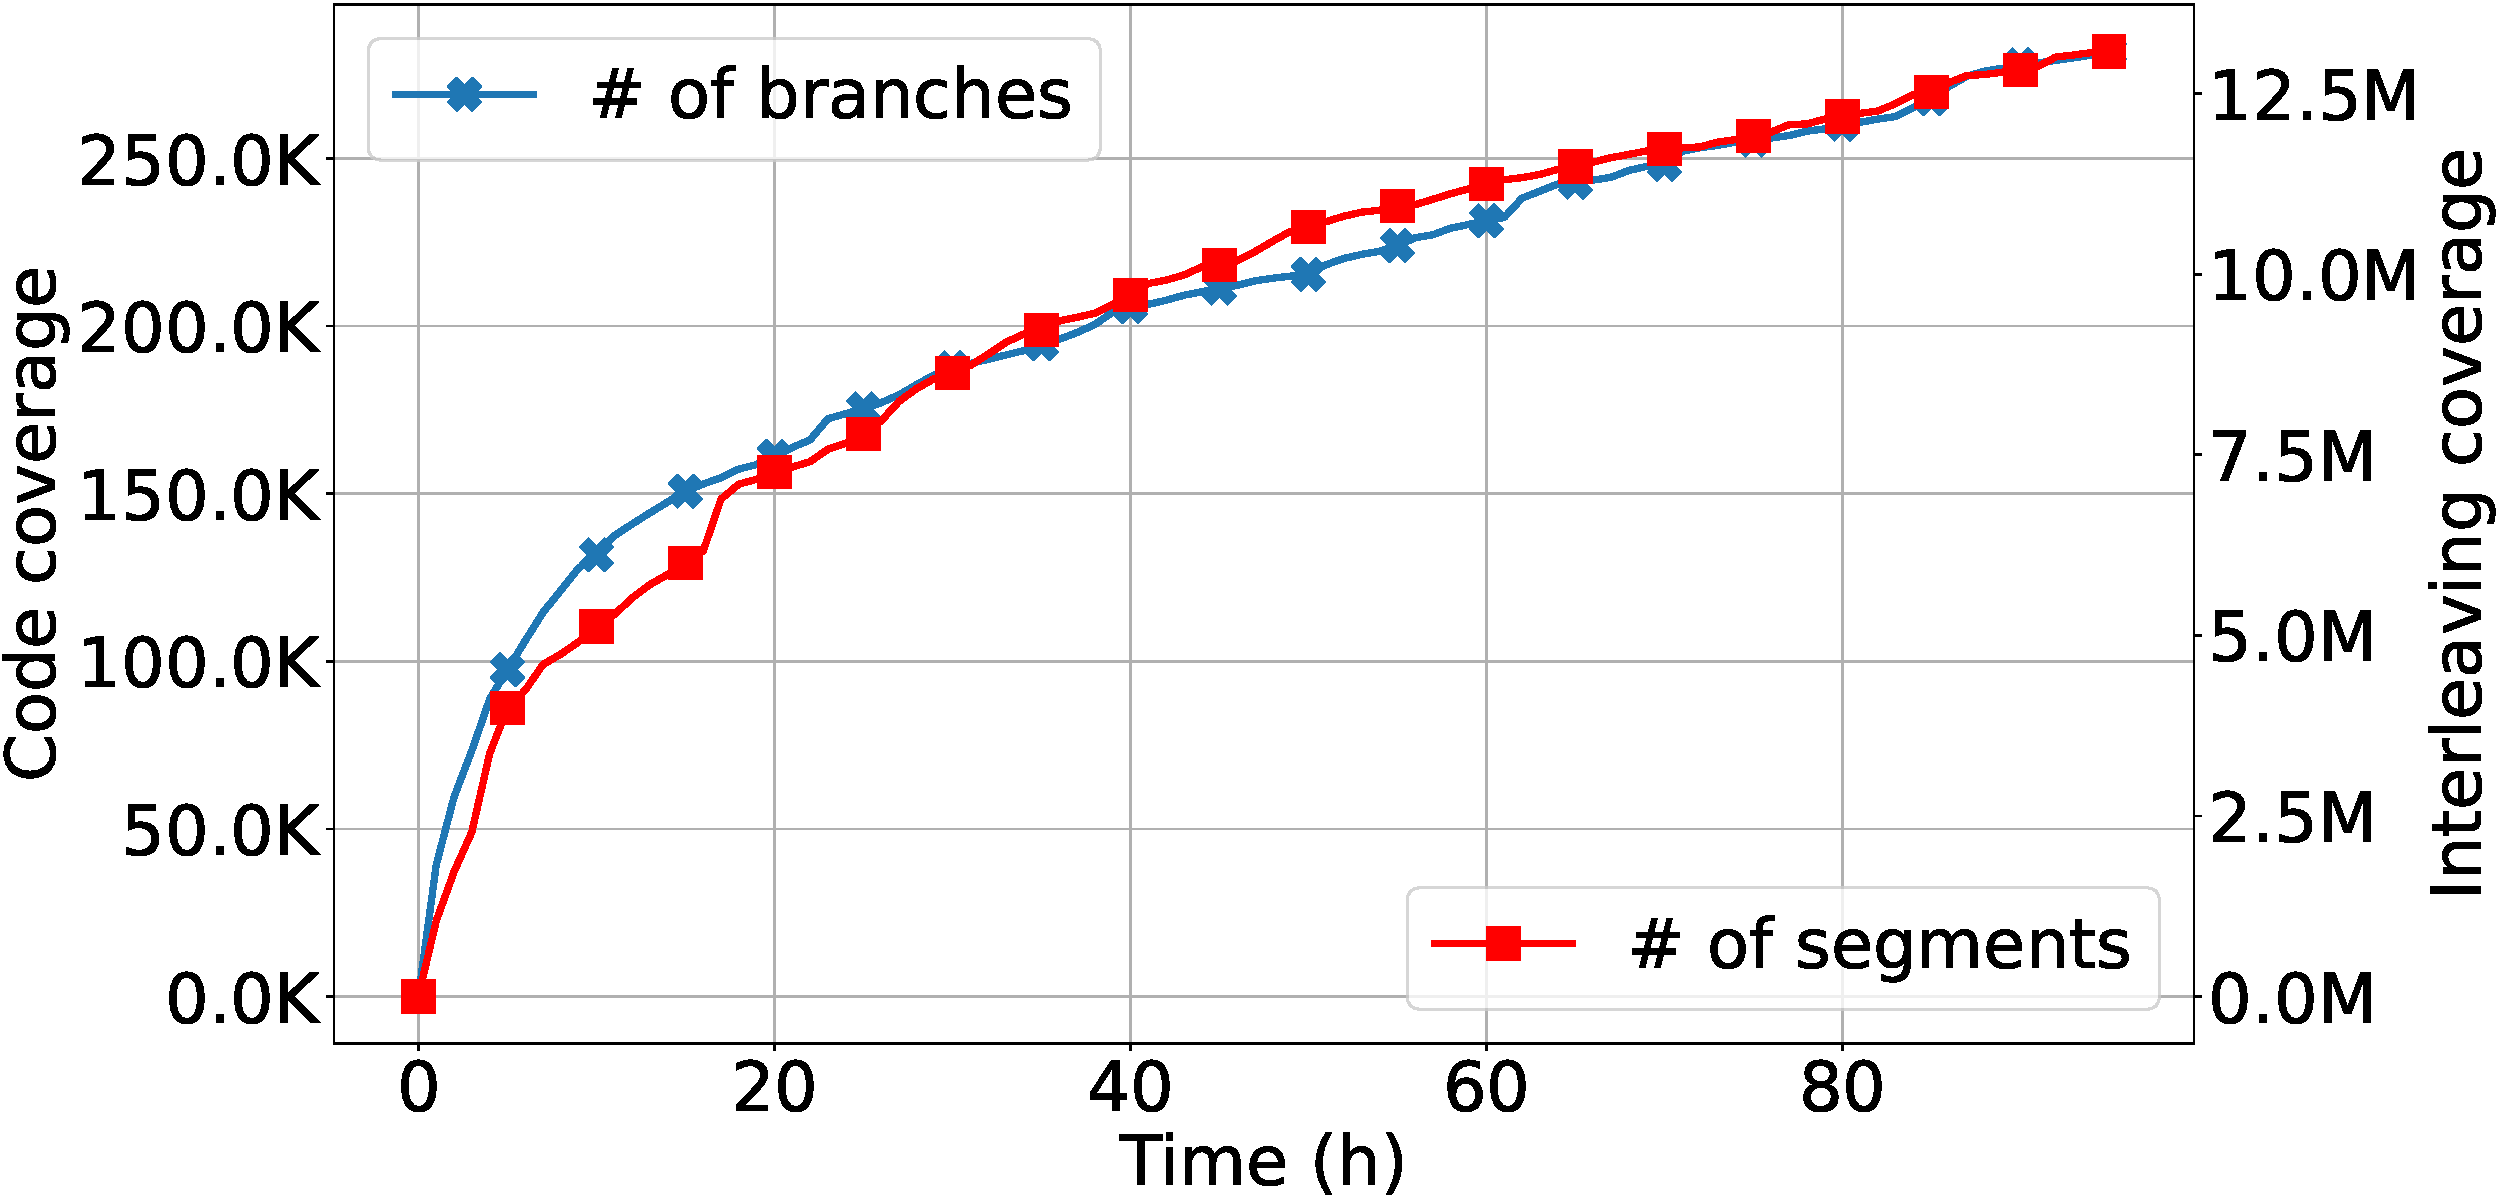
\includegraphics[width=\linewidth]{fig/coverage_graph-crop.pdf}
  \caption{Coverage growth of \sys.\dr{TODO: rewording legend and axis}}
  \label{fig:eval:coverage}
\end{figure}
%
Since coverage metrics are the paramount performance metric of
fuzzing, we first measure the coverage growth for both code coverage
(\ie, the number of taken branches) and interelaving coverage (\ie,
the number of observed interleaving segments) during 100 hours of
fuzzing.

As shown in \autoref{fig:eval:coverage}, there is a notable difference
in scale between code coverage and interleaving coverage.
%
While the number of taken branches just reaches to 300K, the number of
interleaving segments is over 20M. Thus, the scale of interleaving
coverage is more than 66 times of code coverage during our evaluation.
%
This result follows the conventional belief that the search space of
thread interleaving is very large.

One thing to note about this scale difference is that storing
interleaving segment coverage consumes more memory than storing branch
coverage.
%
In our implementation, both branch coverage and interleaving segment
coverage are represented as hash tables where each element is
8-byte. Therefore, storing interleaving segment coverage consumes
about 180\MB while storing branch coverage requires 2\MB.
%
While this high memory pressure is definitely a downside of
interleaving segment coverage, we can consider this as a traditional
space-time tradeoff~\cite{spacetimetradeoff}; we invest \textit{more
  memory} to discover concurrency bugs \textit{faster}.
%
% In addition, considering each VM is equipped with 8\GB memory, it is
% endurable for the fuzzer to store interleaving segment coverage using
% 180\MB (or even using ten times of 180\MB).


\PP{Coverage growth without thread scheduling control}
%
In order to understand the effectiveness of \dr{}



\PP{Fuzzing throughput.}
%
\begin{table}[t]
  \small
  \centering
  \resizebox{0.65\linewidth}{!}{
\begin{tabular}{l l l}
  \toprule
  \sys & \texttt{Syzkaller} & \texttt{Syzkaller-memtrace} \\
  \midrule
  4.55 & 8.40 & 4.74 \\
  \bottomrule
\end{tabular}
}



% syzkaller: 30234
% syzkaller-memtrace: 17608
% c2fuzz: 16386


%%% Local Variables:
%%% mode: latex
%%% TeX-master: "../p"
%%% End:

  \caption{Fuzzing throughput (\# of exec/s) of \sys and
    \texttt{Syzkaller}. \texttt{Syzkaller-memtrace} indicates
    throughput of \texttt{Syzkaller} with memory access tracing
    enabled.}
  \label{table:throughput}
\end{table}
%
All \sys's mechanisms provide benefits in finding concurrency bugs
with a cost of additional overheads and throughput degradation.
%
To comprehend the trade-off, we measure the fuzzing throughput of \sys
and compare it with the \texttt{Syzkaller}'s throughput.
%
In order to experiment in the same environment, we measure throughput
with an empty set of seed. And because both \texttt{Syzkaller} and
\sys restart VMs after an hour of fuzzing, we measure throughput in an
hour of execution in order to eliminate noises caused by, for example,
VM rebooting or kernel crashes.



\autoref{table:throughput} shows the result. As expected, \sys shows
the lower throughput than \texttt{Syzkaller}. In particular, the
\sys's throughput is about 54\% of the \texttt{Syzkaller}'s
throughput.
%
To further understand why the \sys's throughput is degraded, we
additionally measure throughput of \texttt{Syzkaller} with memory
access tracing enabled~(\autoref{ss:instrumentation}) (but not making
use of it).
%
As shown in the \texttt{Syzkaller-memtrace} column in
\autoref{table:throughput}, it shows the throughput similar to that of
\sys; the \texttt{Syzkaller-memtrace}'s throughput is just 4.1\%
higher than the throughput of \sys.


These results indicate that the throughput of \sys is mainly degraded
by the heavy instrumentation to trace memory accesses.
%
However, as KRace~\cite{krace} states, it can be understandable as a
trade-off between throughput and input quality.
%
In the fuzzer's perspective, while tracking memory accesses has
negative impacts on throughput, it provides a higher chance for a
fuzzer to execute more interesting inputs (\ie, interesting thread
interleaving) and not to waste computing resources.
%
The effectiveness of high input quality is pronounced in
\autoref{ss:comparison}, showing \sys can discover concurrency bugs
extremely fast.




\PP{Per-input execution time}
%
\begin{table}[t]
  \centering
  \resizebox{\linewidth}{!}{
  \begin{tabular}{l l l l l l }
    \toprule
    & & \multicolumn{2}{c}{Comp. overhead~(\autoref{s:design})} & \multicolumn{2}{c}{Runtime overhead~(\autoref{s:impl})} \\
    \midrule
    Total & \thead{Exec.\\syscall} & \thead{Tracking\\coverage\\(\autoref{ss:coverage})} & \thead{Interleaving\\search\\(\autoref{ss:scheduler})} & \thead{Tracing\\accsses\\(\autoref{ss:instrumentation})}  & \thead{Thread\\scheduling\\(\autoref{ss:engine})}  \\
    \midrule
    267.2 & 107.6  & 8.9 & 17.2 & 90.7 & 42.8 \\
    \bottomrule
  \end{tabular}
}

% temporary
% c2fuzz
%  execute            241116156.29326048
%  mutate             17231640.620481927
%  post               8858728.732142856
% syzkaller           107640966.51956181
% syzkaller-memtrace  198337534.77521613

%%% Local Variables:
%%% mode: latex
%%% TeX-master: "../p"
%%% End:

  \caption{\dr{rewrite:} Elapsed time (ms) for executing one input.}
  \label{table:elapsedtime}
\end{table}
%
\dr{Rewrite}
%
To closely examine \sys's overheads, we measure the elapsed time for
an iteration of a fuzzing loop, and break down the elapsed time into
time taken by computation (\ie, incurred by generating a schedule and
checking new coverage) and execution of an input.
%
It is worth noting that executing an input entails two overheads for
controling thread interleaving and tracing memory accesses. To
identify how much each overhead occupies, we disable XXX and YYY, and
again measure elapsed times.
%
For each measurement, we run 10 thousands times and take an average.

\autoref{table:elapsedtime} shows the result. When executing the
input, the computational overhead is approximately 9\% of the total
elapsed time. In contrast, executing an input takes the longest time
out of the total elapsed time.
\dr{}



\subsection{Comparison with prior approaches}
\label{ss:comparison}

\begin{table}[t]
  \resizebox{\linewidth}{!}{
  \begin{tabular}{l l l l l}
    \toprule
    \textbf{Bug ID} & \textbf{Subsystem} & \textbf{Crash Type} & \textbf{Reference} \\
    \midrule
    CVE-2016-8655~\cite{cve20168655} & net/packet & use-after-free access & \cite{razzer, exprace} \\
    \midrule
    CVE-2017-2636~\cite{cve20172636} & drivers/tty & double-free & \cite{razzer, exprace} \\
    \midrule
    CVE-2017-7533~\cite{cve20177533} & fs/notify & slab-out-of-bound access & \cite{exprace} \\
    \midrule
    CVE-2017-17712~\cite{cve201717712} & net/ipv4 & uninitialized access & \cite{razzer, exprace} \\
    \midrule
    CVE-2019-1999~\cite{cve20191999} & drivers/android & double-free & \cite{exprace} \\
    \midrule
    CVE-2019-2025~\cite{cve20192025} & drivers/android & use-after-free access & \cite{exprace}  \\
    \midrule
    CVE-2019-6974~\cite{cve20196974} & virt/kvm & use-after-free access & \cite{exprace} \\
    \midrule
    CVE-2019-11486~\cite{cve201911486} & drivers/tty & use-after-free access & \cite{exprace} \\
    \midrule
    69e16d01d1de~\cite{snowboardbug} & net/l2tp & NULL dereference & \cite{snowboard} \\
    \bottomrule
  \end{tabular}
}

%%% Local Variables:
%%% mode: latex
%%% TeX-master: "../"
%%% End:

  \centering
  \caption{Known concurrency bugs that are studied in previous works,
    MoonShine~\cite{moonshine}, Razzer~\cite{razzer},
    ExpRace~\cite{exprace}, FUZE~\cite{fuze}, and
    Snowboard~\cite{snowboard}.}
  \label{table:knownbugs}
\end{table}

We compare \sys against various prior approaches, KRace~\cite{krace},
Snowboard~\cite{snowboard} to demonstrate the performance improvement
in discovering concurrency bugs.

\PP{Bug selection}
%
\autoref{table:knownbugs} represents concurrency bugs we use for the
comparison study.
%
For fair comparisons, we select kernel concurrency bugs that are used
to evaluate previous studies on kernel concurrency bugs~\cite{exprace,
  razzer, snowboard, moonshine, fuze}.
%
Specifically, among concurrency bugs used in previous studies, we
select ones that their exploits are publicly available such that we
can make use of them for our evaluation.
%
Although the exploit of \texttt{69e16d01d1de}~\cite{snowboardbug} is
not publicly available, we successfully reproduce the concurrency bug
from the description in the Snowboard~\cite{snowboard} paper.
%
Whereas, even though KRace~\cite{krace} studies kernel concurrency
bugs (\ie, data races), we do not have access to concurrency bugs that
the authors use to evaluate KRace, and we exclude two concurrency bugs
(\ie, CVE-2019-1999~\cite{cve20191999} and
CVE-2019-2025~\cite{cve20192025}) used by ExpRace~\cite{exprace}
because \dr{XXX}.



\PP{Kernel preparation}
%
Since concurrency bugs in \autoref{table:knownbugs} are introduced,
found, and fixed at different times, it is hard to find a kernel
version that is vulnerable to all listed concurrency bugs.
%
Therefore, we inject the concurrency bugs into the Linux kernel
version v6.0-rc7 by reverting patches fixing the concurrency bugs.




\PP{Comparison methodology}
%
\begin{figure}[t]
  \caption{A multi-thread input that causes
    CVE-2017-17712~\cite{cve201717712}. The concurrency bugs may
    manifests if two system calls in bold exeucte a specific thread
    interleaving.}
  \label{fig:multithreadinput}
\end{figure}
%
Arguably, the most straightforward metric to compare fuzzing
techniques is the elapsed time until concurrency bugs are discovered.
%
However, the elapsed time heavily depends on the randomness;
\dr{because a fuzzer generates an input program very randomly, it is
  possible that one fuzzer quickly generates an input program that
  causes a concurrency bug, while another fuzzer takes very long time
  to generate the input program}.

In order to minimize the impact of the randomness and to concentrate
on the performance impact of scheduling mechanisms, we predefine a
multi-thread input as shown in \autoref{fig:multithreadinput}, and let
a fuzzer repeatedly execute the given multi-thread input without
generating new inputs nor mutating syscalls in the given input.

In addition, previous fuzzing approaches


\PP{}
%
\begin{figure*}[t]
  \centering
  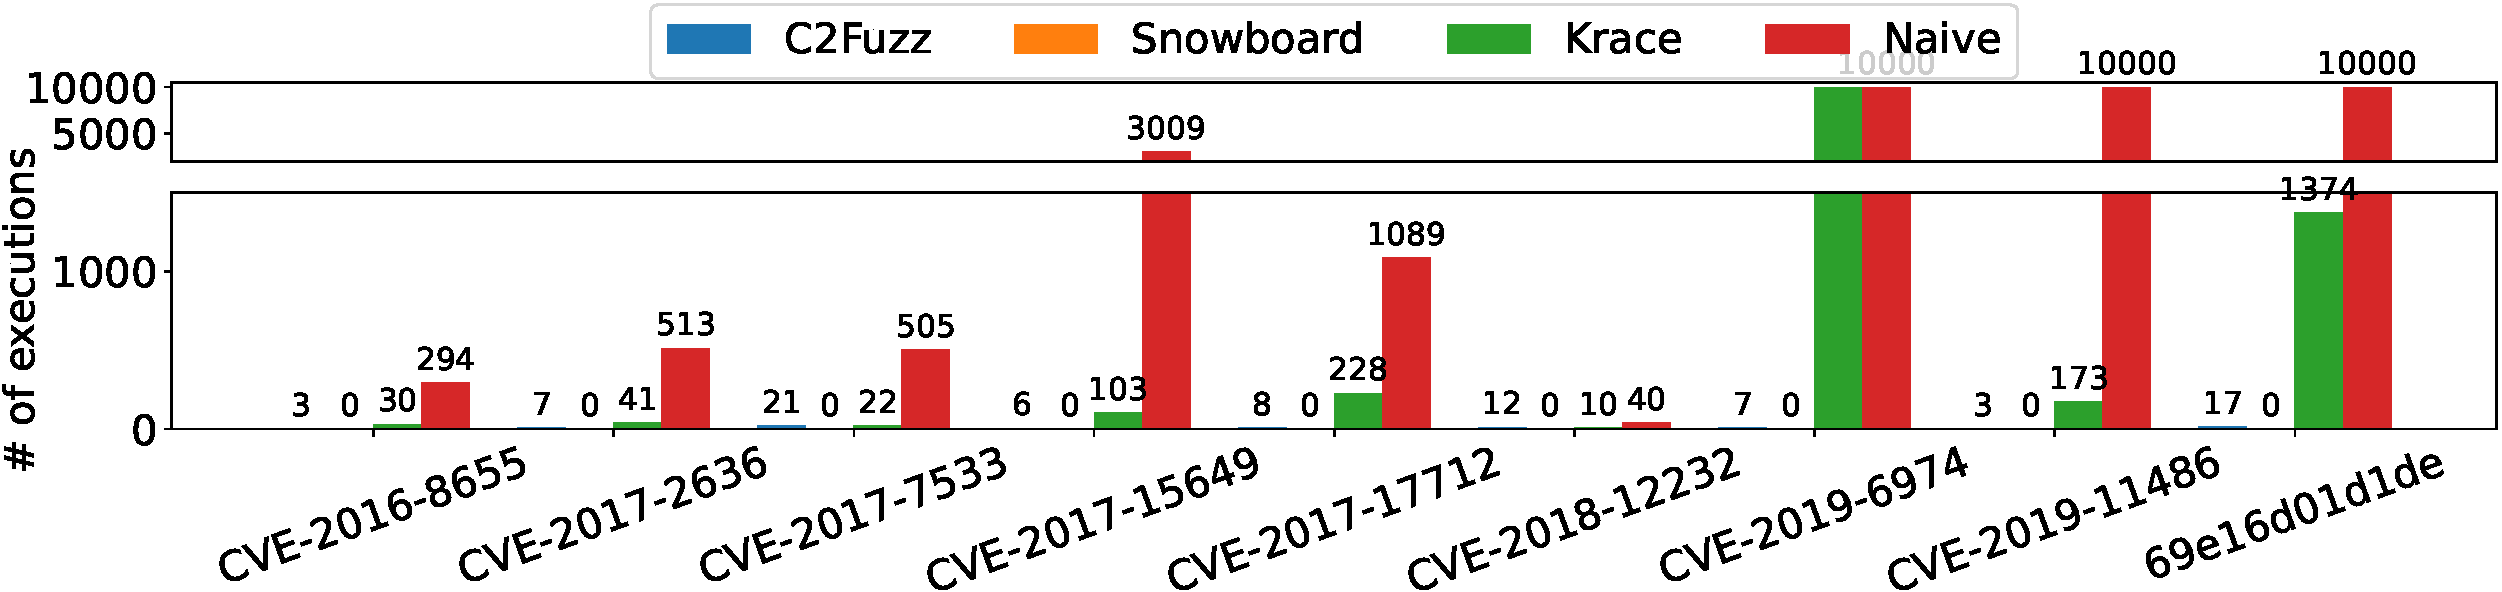
\includegraphics[width=\linewidth]{fig/comparison_graph-crop.pdf}
  \caption{\dr{WIP. Snowboard is not implemented yet} \dr{table is better?}}
  \label{fig:eval:comparison}
\end{figure*}
%

\autoref{fig:eval:comparison} shows the comparison result.
%



The difficulty of triggering a concurrency bug is different.






% Single
% cve-2016-8655 O
% cve-2017-15649 O
% cve-2017-17712 X
% cve-2017-2636 X
% cve-2017-7533 X
% cve-2019-6974 X
% cve-2019-11486 X
% 69e16d01d1d O



%%% Local Variables:
%%% mode: latex
%%% TeX-master: "p"
%%% End:
